%%%%%%%%%%%%%%%%% DO NOT CHANGE HERE %%%%%%%%%%%%%%%%%%%% {
\documentclass[12pt,letterpaper]{article}
\usepackage{fullpage}
\usepackage[top=2cm, bottom=4.5cm, left=2.5cm, right=2.5cm]{geometry}
\usepackage{amsmath,amsthm,amsfonts,amssymb,amscd}
\usepackage{lastpage}
\usepackage{enumerate}
\usepackage{fancyhdr}
\usepackage{mathrsfs}
\usepackage{xcolor}
\usepackage{graphicx}
\usepackage{subcaption}
\usepackage{listings}
\usepackage{hyperref}
\usepackage{tikz}
\usetikzlibrary{positioning,shapes,arrows}
\usetikzlibrary[calc]

\hypersetup{%
  colorlinks=true,
  linkcolor=blue,
  linkbordercolor={0 0 1}
}

\setlength{\parindent}{0.0in}
\setlength{\parskip}{0.05in}
%%%%%%%%%%%%%%%%%%%%%%%%%%%%%%%%%%%%%%%%%%%%%%%%%%%%%%%%%% }

%%%%%%%%%%%%%%%%%%%%%%%% CHANGE HERE %%%%%%%%%%%%%%%%%%%% {
\newcommand\course{CSI5138[F]: Intro: DL/RL}
\newcommand\semester{Fall 2019}
\newcommand\hwnumber{2}                 % <-- ASSIGNMENT #
\newcommand\NetIDa{Ao Zhang, 0300039680}           % <-- First Author
\newcommand\NetIDb{Lingfeng Zhang, 0300134245}           % <-- Second Author #
%%%%%%%%%%%%%%%%%%%%%%%%%%%%%%%%%%%%%%%%%%%%%%%%%%%%%%%%%% }

%%%%%%%%%%%%%%%%% DO NOT CHANGE HERE %%%%%%%%%%%%%%%%%%%% {
\pagestyle{fancyplain}
\headheight 35pt
\lhead{\NetIDa}
\lhead{\NetIDa\\\NetIDb}                 
\chead{\textbf{\Large Assignment \hwnumber}}
\rhead{\course \\ \semester}
\lfoot{}
\cfoot{}
\rfoot{\small\thepage}
\headsep 1.5em
%%%%%%%%%%%%%%%%%%%%%%%%%%%%%%%%%%%%%%%%%%%%%%%%%%%%%%%%%% }

% Define block styles
\tikzstyle{sum} = [circle, draw, minimum size=1em]
\tikzstyle{mul} = [rectangle, draw, minimum size=1em]
\tikzstyle{var} = [text width=1em, text centered, minimum size=1em]
\tikzstyle{sig} = [diamond, draw, fill=blue!20, minimum size=1em]
\tikzstyle{sqsum} = [circle, draw, fill=blue!20, minimum size=1em]
\tikzstyle{line} = [draw, -latex']

\begin{document}

\section{Question 1}

Since the question asks us to hand-derive back propagation of the defined neural network architecture, a forward graph is firstly built as Figure~\ref{fig:forward} for showing the relationships between all those nodes.
\begin{figure}[h]
    \centering
    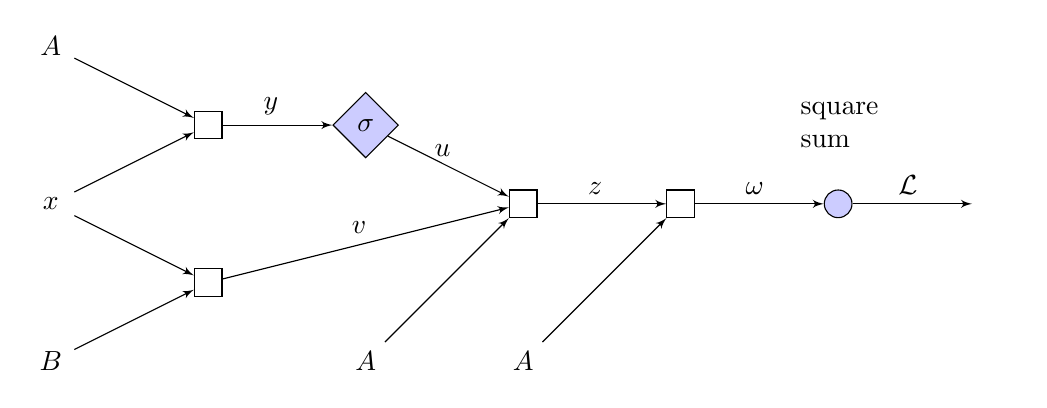
\begin{tikzpicture}[node distance = 2cm, auto]
        % Place nodes
        \node at (0, 0) [var] (B) {$B$};
        \node at (0, 2) [var] (x) {$x$};
        \node at (0, 4) [var] (A) {$A$};
        \node at (2, 1) [mul] (mul1) {};
        \node at (2, 3) [mul] (mul2) {};
        \node at (4, 3) [sig] (sig) {$\sigma$};
        \node at (4, 0) [var] (A2) {$A$};
        \node at (6, 0) [var] (A3) {$A$};
        \node at (6, 2) [mul] (mul3) {};
        \node at (8, 2) [mul] (mul4) {};
        \node at (10, 2) [sqsum] (sqsum) {};
        \node at (9.7, 3) [var] (sqname) {square sum};
        \node at (12, 2) [var] (end) {};
        
        % Draw edges
        \path [line] (A) -- node [text width=1em,midway,above ] {} (mul2);
        \path [line] (x) -- node [text width=1em,midway,above ] {} (mul2);
        \path [line] (x) -- node [text width=1em,midway,above ] {} (mul1);
        \path [line] (B) -- node [text width=1em,midway,above ] {} (mul1);
        \path [line] (mul2) -- node [text width=1em,midway,above ] {$y$} (sig);
        \path [line] (sig) -- node [text width=1em,midway,above ] {$u$} (mul3);
        \path [line] (mul1) -- node [text width=1em,midway,above ] {$v$} (mul3);
        \path [line] (mul3) -- node [text width=1em,midway,above ] {$z$} (mul4);
        \path [line] (A2) -- node [text width=1em,midway,above ] {} (mul3);
        \path [line] (A3) -- node [text width=1em,midway,above ] {} (mul4);
        \path [line] (mul4) -- node [text width=1em,midway,above ] {$\omega$} (sqsum);
        \path [line] (sqsum) -- node [text width=1em,midway,above ] {$\mathcal{L}$} (end);
    \end{tikzpicture}
    \caption{\small Forward graph $\mathcal{G}$.}
    \label{fig:forward}
\end{figure}

Also, as mentioned in the lecture, the back propagation is the dual function of the forward gradient propagation. Therefore, in order to get the back propagation gradient, we firstly should derive the forward gradient graph, shown as Figure~\ref{fig:gradient}

\begin{figure}[h]
\centering
    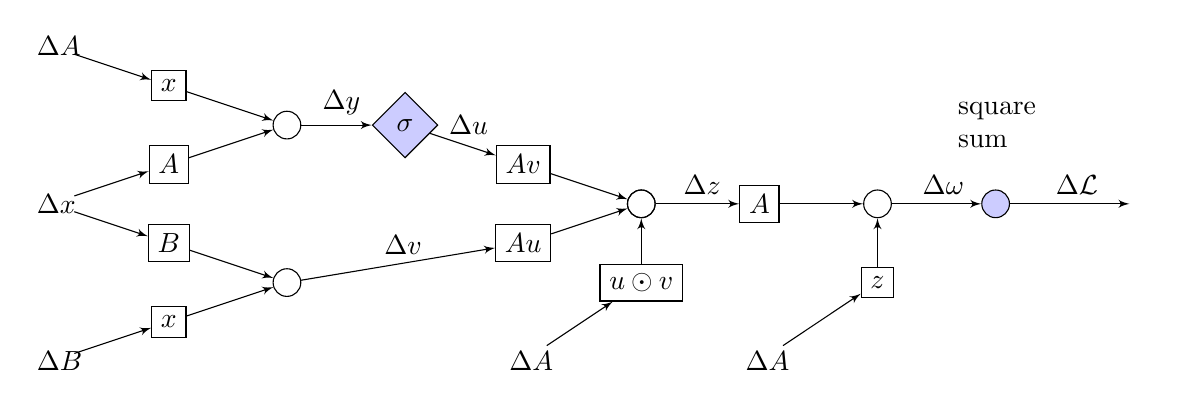
\begin{tikzpicture}[node distance = 2cm, auto]
        % Place nodes
        \node at (0, 0) [var] (B) {$\Delta B$};
        \node at (0, 2) [var] (x) {$\Delta x$};
        \node at (0, 4) [var] (A) {$\Delta A$};
        \node at (1.5, 3.5) [mul] (mul1) {$x$};
        \node at (1.5, 2.5) [mul] (mul2) {$A$};
        \node at (1.5, 1.5) [mul] (mul3) {$B$};
        \node at (1.5, 0.5) [mul] (mul4) {$x$};
        \node at (3, 1) [sum] (sum1) {};
        \node at (3, 3) [sum] (sum2) {};
        \node at (4.5, 3) [sig] (sig) {$\sigma$};
        \node at (6, 2.5) [mul] (mul5) {$Av$};
        \node at (6, 1.5) [mul] (mul6) {$Au$};
        \node at (7.5, 2) [sum] (sum3) {};
        \node at (7.5, 1) [mul] (mul7) {$u \odot v$};
        \node at (6, 0) [var] (A2) {$\Delta A$};
        \node at (9, 2) [mul] (mul8) {$A$};
        \node at (7.5, 2) [sum] (sum3) {};
        \node at (10.5, 2) [sum] (sum4) {};
        \node at (10.5, 1) [mul] (mul9) {$z$};
        \node at (9, 0) [var] (A3) {$\Delta A$};
        \node at (12, 2) [sqsum] (sqsum) {};
        \node at (11.7, 3) [var] (sqname) {square sum};
        \node at (14, 2) [var] (end) {};
        
        % Draw edges
        \path [line] (A) -- node [text width=1em,midway,above ] {} (mul1);
        \path [line] (x) -- node [text width=1em,midway,above ] {} (mul2);
        \path [line] (x) -- node [text width=1em,midway,above ] {} (mul3);
        \path [line] (B) -- node [text width=1em,midway,above ] {} (mul4);
        \path [line] (mul1) -- node [text width=1em,midway,above ] {} (sum2);
        \path [line] (mul2) -- node [text width=1em,midway,above ] {} (sum2);
        \path [line] (mul3) -- node [text width=1em,midway,above ] {} (sum1);
        \path [line] (mul4) -- node [text width=1em,midway,above ] {} (sum1);
        \path [line] (sum2) -- node [text width=1em,midway,above ] {$\Delta y$} (sig);
        \path [line] (sig) -- node [text width=1em,midway,above ] {$\Delta u$} (mul5);
        \path [line] (sum1) -- node [text width=1em,midway,above ] {$\Delta v$} (mul6);
        \path [line] (mul5) -- node [text width=1em,midway,above ] {} (sum3);
        \path [line] (mul6) -- node [text width=1em,midway,above ] {} (sum3);
        \path [line] (mul7) -- node [text width=1em,midway,above ] {} (sum3);
        \path [line] (A2) -- node [text width=1em,midway,above ] {} (mul7); 
        \path [line] (sum3) -- node [text width=1em,midway,above ] {$\Delta z$} (mul8);
        \path [line] (mul8) -- node [text width=1em,midway,above ] {} (sum4);
        \path [line] (mul9) -- node [text width=1em,midway,above ] {} (sum4);
        \path [line] (A3) -- node [text width=1em,midway,above ] {} (mul9);
        \path [line] (sum4) -- node [text width=1em,midway,above ] {$\Delta \omega$} (sqsum);
        \path [line] (sqsum) -- node [text width=1em,midway,above ] {$\Delta \mathcal{L}$} (end);
    \end{tikzpicture}
    \caption{\small Forward Gradient graph $\partial \mathcal{G}$.}
    \label{fig:gradient}
\end{figure}

Now, we could easily get the back propagation graph by transposing forward graph, which is,
\begin{equation*}
    \frac{\partial \mathcal{L}}{\partial \boldsymbol{\theta}} = \big( \partial \mathcal{G} \big)^T
\end{equation*}

Notice that, the parameter $A$ appears $3$ times in the graph. So according to the chain rule, the result of the back propagation gradients w.r.t each parameter are,
\begin{align*}
    \frac{\partial \mathcal{L}}{\partial A} &=  \frac{\partial \mathcal{L}}{\partial \omega} \frac{\partial \omega}{\partial z} \odot \frac{\partial z}{\partial u} \odot \frac{\partial u}{\partial y} \frac{\partial y}{\partial A} + \frac{\partial \mathcal{L}}{\partial \omega} \frac{\partial \omega}{\partial z} \frac{\partial z}{\partial A} + \frac{\partial \mathcal{L}}{\partial \omega} \frac{\partial \omega}{\partial A} \\
    \frac{\partial \mathcal{L}}{\partial B} &= \frac{\partial \mathcal{L}}{\partial \omega} \frac{\partial \omega}{\partial z} \odot \frac{\partial z}{\partial v} \frac{\partial v}{\partial B}
\end{align*}
where, the reason why there appears $\odot$ is that the third function $z = A(u \odot v)$ is the element-wise multiplication.

So, the upper equations are expanded to,

\begin{align*}
    \frac{\partial \mathcal{L}}{\partial A} &= 2\omega Z^T + 2A^T\omega (u \odot v)^T+\sigma(2A^TA^T\omega \odot v)\odot (1 - \sigma(2A^TA^T\omega \odot v))x^T \\
    \frac{\partial \mathcal{L}}{\partial B} &= (2A^TA^T\omega \odot u)x^T
\end{align*}

After implementing in the python code, we produce a random input and the result of the loss function is shown as Figure~\ref{fig:experiment}
\begin{figure}[h]
    \centering
    \includegraphics[width=.6\linewidth]{assignment1_question1.png}
    \caption{\small Results of back propagation.}
    \label{fig:experiment}
\end{figure}

The parameters settings are shown below,
\begin{table}[h]
        \centering
        \vspace{\baselineskip}
        \caption{All relative parameters values.}\label{T:parameters}
      \begin{tabular}{cc}
        \hline
        Parameter & Value\\
        \hline
        N (number of inputs) & 100\\
        K (input dimensions) & 5\\
        optimization & Gradient Descent\\
        \hline
      \end{tabular}
\end{table}

According to the result, we could conclude the gradient based back propagation could make minimize the loss function and make the model learn.

\newpage
\section{Question 2}

For softmax function in this question, K represents K kind of classes and m represents m kind of features for each input x. So $Wx \in \mathbb{R^{K \times 1}}$ means there is a value for each class and softmax(Wx) gives each class with a probability. W is just a symbol, so I use another symbol $F \in \mathbb{R^{K \times K}}$ there. Softmax(Wx) and Softmax(Fx) are in the same hypothesis space, and they have same probability distribution because they can be trained and reached same result finally whether their initialization are same or not.

Due to their distribution are same, expectation can be used to proof this question.

There are two matrix expectation formula which should be introduced.

\begin{align*}
    E(AX) &= AE(X) \\
    E(A+B) &= E(A) + E(B)
\end{align*}

In order to proving the problem, we introduce another $3$ hypothesis,
\begin{align*}
    D &= AC, \,\, A \in \mathbb{R}^{K \times K},  C \in \mathbb{R}^{K \times K}\\
    E &= BC, \,\, B \in \mathbb{R}^{K \times K},  C \in \mathbb{R}^{K \times K}\\
    F &= D + E, \,\, D \in \mathbb{R}^{K \times K},  E \in \mathbb{R}^{K \times K}\\
\end{align*}
where, since $ A \in \mathbb{R}^{K \times K},  B \in \mathbb{R}^{K \times K}, C \in \mathbb{R}^{K \times K}$, according to the linear combination, $D \in \mathbb{R}^{K \times K}$. Similarly, $E \in \mathbb{R}^{K \times K}$ and $F \in \mathbb{R}^{K \times K}$.

From another point of view, since for each member hypothesis in $\mathcal{H}_1$ and $\mathcal{H}_2$ specifies a $p_{Y|X}$, the relationship of the expectation can be derived between D,E,F and A,B,C,

\begin{align*}
    E(Dx) &= E(ACx) \\
        &= AE(Cx) \\
    E(Ex) &= E(BCx) \\
        &= BE(Cx) \\
    E(Fx) &= E((D+E)x) \\
        &= E(Dx + Ex) \\
        &= E(Dx) + E(Ex) \\
        &= AE(Cx) + BE(Cx) \\
        &= (A+B)E(Cx) \\
        &= E((A+B)Cx)
\end{align*}

Due to Softmax(Wx) and Softmax(Fx) have the same distribiton, their expecation are same too.

\begin{align*}
    E(Softmax(Wx)) &= E(Softmax(Fx))
\end{align*}

Softmax use the way of probability to represent expectation, and the way of values can also be represented by expectation,meaning the expectation of Wx and of Fx are same,too.So,
\begin{align*}
    E(Wx) &= E(Fx) \\
        &= E((A+B)Cx)
\end{align*}

Back to the probability way,
\begin{align*}
    E(Softmax(Wx)) &= E(Softmax((A+B)Cx))
\end{align*}

Because Softmax(Wx) and Softmax((A+B)Cx) have same expectation, they have same probability distribution.

Therefore,
\begin{equation*}
    \mathcal{H}_1 = \mathcal{H}_2
\end{equation*}

\newpage
\section{Question 3}

Since the question asks us to define the model first, we will introduce the model we used for the test first.

\subsection{Model Introduction}

\subsubsection*{Soft-max Regression}

Simply, we define the soft-max regression as,
\begin{equation*}
    y = \textbf{softmax}\Big( Wx + b \Big)
\end{equation*}

\subsubsection*{MLP}

The MLP we defined is shown as Figure~\ref{fig:MLP}.

\tikzset{%
  every neuron/.style={
    circle,
    draw,
    minimum size=1.5em
  },
  neuron missing/.style={
    draw=none, 
    scale=4,
    text height=0.333cm,
    execute at begin node=\color{black}$\vdots$
  },
}

\begin{figure}[h]
    \centering
    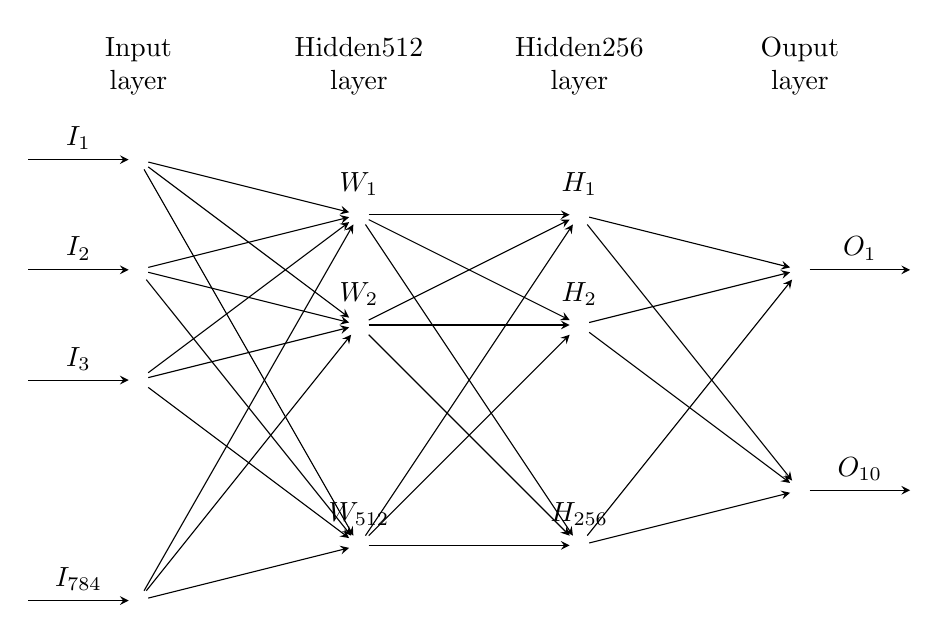
\begin{tikzpicture}[x=1.4cm, y=1.4cm, >=stealth]
    
    \foreach \m/\l [count=\y] in {1,2,3,missing,4}
      \node [every neuron/.try, neuron \m/.try] (input-\m) at (0,2.5-\y) {};
    
    \foreach \m [count=\y] in {1,2,missing,3}
      \node [every neuron/.try, neuron \m/.try ] (hidden1-\m) at (2,2-\y*1) {};
      
    \foreach \m [count=\y] in {1,2,missing,3}
      \node [every neuron/.try, neuron \m/.try ] (hidden2-\m) at (4,2-\y*1) {};
    
    \foreach \m [count=\y] in {1,missing,2}
      \node [every neuron/.try, neuron \m/.try ] (output-\m) at (6,1.5-\y) {};
    
    \foreach \l [count=\i] in {1,2,3,784}
      \draw [<-] (input-\i) -- ++(-1,0)
        node [above, midway] {$I_{\l}$};
    
    \foreach \l [count=\i] in {1,2,{512}}
      \node [above] at (hidden1-\i.north) {$W_{\l}$};
      
    \foreach \l [count=\i] in {1,2,{256}}
      \node [above] at (hidden2-\i.north) {$H_{\l}$};
    
    \foreach \l [count=\i] in {1,{10}}
      \draw [->] (output-\i) -- ++(1,0)
        node [above, midway] {$O_{\l}$};
    
    \foreach \i in {1,...,4}
      \foreach \j in {1,...,3}
        \draw [->] (input-\i) -- (hidden1-\j);
    
    \foreach \i in {1,...,3}
      \foreach \j in {1,...,3}
        \draw [->] (hidden1-\i) -- (hidden2-\j);
        
    \foreach \i in {1,...,3}
      \foreach \j in {1,...,2}
        \draw [->] (hidden2-\i) -- (output-\j);
    
    \foreach \l [count=\x from 0] in {Input, Hidden512, Hidden256, Ouput}
      \node [align=center, above] at (\x*2,2) {\l \\ layer};
    \end{tikzpicture}
\caption{\small MLP model for the question 3.}
    \label{fig:MLP}
\end{figure}

We set two hidden layers, with first hidden layers having $512$ nodes and second hidden layer having $256$ nodes.

The mathematical model could be expressed as,
\begin{align*}
    \hat{Y} &= \sigma \Big( W_3 \cdot \text{relu} \Big( W_2 \cdot \text{relu} \big( W_1 X + b_1 \big) + b_2 \Big) + b_3 \Big)
\end{align*}
where,
\begin{equation*}
    X \in \mathbb{R}^{N \times 784}, \,\, W_1 \in \mathbb{R}^{784 \times 512}, \,\, W_2 \in \mathbb{R}^{512 \times 256}, \,\, W_3 \in \mathbb{R}^{256 \times 10} \\
    b_1 \in \mathbb{R}^{512}, \,\, b_2 \in \mathbb{R}^{256}, \,\, b_3 \in \mathbb{R}^{10}
\end{equation*}

\subsubsection*{CNN}

The structure of CNN used in this assignment could be seen as Figure~\ref{fig:CNN}.
\begin{figure}[h]
    \centering
    \includegraphics[width=.9\linewidth]{CNN.jpg}
    \caption{\small CNN model for the question 3.}
    \label{fig:CNN}
\end{figure}

\subsubsection*{Other parameters settings}

Since we want to find out the influences of batch normalization and drop out on different models, we set all other parameters as the same during the whole training process. The parameter settings is shown below,
\begin{table}[h]
        \centering
        \vspace{\baselineskip}
        \caption{All relative parameters values.}\label{T:parameters}
      \begin{tabular}{cc}
        \hline
        Parameter & Value\\
        \hline
        learning rate & 0.001\\
        batch size & 500\\
        epoches &  20\\
        dropout rate &  0.5\\
        learning rate decay coefficient &  0.96\\
        learning rate decay steps &  100\\
        optimization method &  Adam\\
        loss function &  cross entropy\\
        \hline
      \end{tabular}
\end{table}

\subsection{Experiments and Conclusion}

In the following section, we will first compare the results of all three models on the loss function values and the accuracies respectively. Then we will dive into the influence of batch normalization and dropout on each model separately. A brief conclusion will be drawn after each comparison. And hopefully, we could be able to cover the main features of each plot.

\subsubsection{Comparison between $3$ models}

The results of the training loss values and validation accuracies are shown as Figure~\ref{fig:all_models}
\begin{figure}[h]
\centering
\begin{subfigure}{.49\textwidth}
  \centering
  \includegraphics[width=.95\linewidth]{allmodels_acc.png}
  \caption{\small Accuracy of the validation set of each model.}
  \label{fig:sub1}
\end{subfigure}%
\begin{subfigure}{.49\textwidth}
  \centering
  \includegraphics[width=.95\linewidth]{allmodels_loss.png}
  \caption{\small Training loss values of each model.}
  \label{fig:sub2}
\end{subfigure}
\caption{\small Results on training set and validation during the whole training process of $3$ models.}
\label{fig:all_models}
\end{figure}

Some predominant characters could be observed as: The loss function of CNN and MLP converge extremely faster than soft-max regression; For the accuracy, CNN is greater than MLP. But they both dramatically outperform the soft-max regression. Several reasons for the phenomenon above could be concluded as,
\begin{itemize}
    \item Since the parameters sizes of both MLP and CNN are significantly greater than that of soft-max regression, they could naturally outperform the soft-max regression model.
    \item Though the parameters sizes of MLP and CNN themselves differ slightly, the main reason why CNN could outperform MLP may not involve the parameters size. One possible reason is that the feature maps extracted from CNN may give more intuitive information about the differences between different classes. Thus, it could make the model predict better.
\end{itemize}

\subsubsection{Influence of Batch Normalization}

According to the result in the first section, we can easily find out that different models have different performances, and the scope of the plots are different too. Therefore, in order to show the difference of each model with and without batch normalization, we separate the plots according to the models.

The results on the accuracies and loss values are shown as Figure~\ref{fig:BN}.

\begin{figure}[h]
    \begin{subfigure}{0.32\textwidth}
    \includegraphics[width=\linewidth]{CNN_BN_acc.png}
    \caption{\small Influence of BN on accuracy of CNN} \label{fig:a}
    \end{subfigure}\hspace*{\fill}
    \begin{subfigure}{0.32\textwidth}
    \includegraphics[width=\linewidth]{MLP_BN_acc.png}
    \caption{\small Influence of BN on accuracy of MLP} \label{fig:b}
    \end{subfigure}
    \begin{subfigure}{0.32\textwidth}
    \includegraphics[width=\linewidth]{softmax_BN_acc.png}
    \caption{\small Influence of BN on accuracy of soft-max} \label{fig:b}
    \end{subfigure}
    
    \medskip
    \begin{subfigure}{0.32\textwidth}
    \includegraphics[width=\linewidth]{CNN_BN_loss.png}
    \caption{\small Influence of BN on loss of CNN} \label{fig:c}
    \end{subfigure}\hspace*{\fill}
    \begin{subfigure}{0.32\textwidth}
    \includegraphics[width=\linewidth]{MLP_BN_loss.png}
    \caption{\small Influence of BN on loss of MLP} \label{fig:d}
    \end{subfigure}
    \begin{subfigure}{0.32\textwidth}
    \includegraphics[width=\linewidth]{softmax_BN_loss.png}
    \caption{\small Influence of BN on loss of soft-max} \label{fig:d}
    \end{subfigure}
    \caption{Influence of Batch Normalization on $3$ models.} \label{fig:BN}
\end{figure}

As the question requests, we will analyse the features of the graphs of each model individually in the following part.
\begin{itemize}
    \item \textbf{For CNN}: we can observe that the performance after batch normalization(BN) goes a little bit higher than before BN within $1200$ training steps. Meanwhile, the loss value after BN also converges faster than before BN. After about $1200$ steps, they both converge to the same level. Potential reasons for this could be seen as: since the BN could actually improve the ability of model to deal with covariance shift, it could help the training process to find the optimal solution faster. While, the training dataset for this specific task is large enough, which results the same performance when the training process goes further.
    \item \textbf{For MLP}: obviously, from testing accuracy, BN significantly improves the performance of the model, while the loss value during the whole training process remains the same. The result basically follows the theory we learnt from the class, that is the BN not only helps the model learn faster, but also helps increase the accuracy of the prediction.
    \item \textbf{For soft-max}: though the loss function remains the same before and after BN, it is weird to see that the performance after BN is actually worse than before. I think one of the possible reasons is that, since the soft-max regression only has one layer before gating function, the actual prediction probability distribution would be changed when we apply BN on the model. It sabotages the true prediction distribution that the original model could possibly have. Therefore, it drives the accuracy away when after 500 training steps.
\end{itemize}


\subsubsection{Influence of Dropout}

Also, in this section, we will draw the conclusion with respect to each model. All of the results is shown as Figure~\ref{fig:Drop}
\begin{figure}[h]
    \begin{subfigure}{0.32\textwidth}
    \includegraphics[width=\linewidth]{CNN_dropout_acc.png}
    \caption{\small Influence of dropout on accuracy of CNN} \label{fig:a}
    \end{subfigure}\hspace*{\fill}
    \begin{subfigure}{0.32\textwidth}
    \includegraphics[width=\linewidth]{MLP_dropout_acc.png}
    \caption{\small Influence of dropout on accuracy of MLP} \label{fig:b}
    \end{subfigure}
    \begin{subfigure}{0.32\textwidth}
    \includegraphics[width=\linewidth]{softmax_dropout_acc.png}
    \caption{\small Influence of dropout on accuracy of soft-max} \label{fig:b}
    \end{subfigure}
    
    \medskip
    \begin{subfigure}{0.32\textwidth}
    \includegraphics[width=\linewidth]{CNN_dropout_loss.png}
    \caption{\small Influence of dropout on loss of CNN} \label{fig:c}
    \end{subfigure}\hspace*{\fill}
    \begin{subfigure}{0.32\textwidth}
    \includegraphics[width=\linewidth]{MLP_dropout_loss.png}
    \caption{\small Influence of dropout on loss of MLP} \label{fig:d}
    \end{subfigure}
    \begin{subfigure}{0.32\textwidth}
    \includegraphics[width=\linewidth]{softmax_dropout_loss.png}
    \caption{\small Influence of dropout on loss of soft-max} \label{fig:d}
    \end{subfigure}
    \caption{Influence of Dropout on $3$ models.} \label{fig:Drop}
\end{figure}

The conclusions would be,
\begin{itemize}
    \item \textbf{For CNN}: since the Convolutional Kernel itself could not be applied with dropout, the only way to do the dropout in the model is the dropout in the last layer(normal linear layer with soft-max gating function). Therefore, as we can see, the dropout itself does not influence the model at all. This basically agrees with our expectation.
    \item \textbf{For MLP}: dropout is used in every single layer of this model. As a result, the accuracy of the model after dropout shows promising improvement than before dropout. The loss function remains the same during the whole process. This is because the dropout, acting as a regularizer, effectively improve the ability of model to deal with the noise. This basically follows the theory we learnt from the class.
    \item \textbf{For soft-max}: apparently, dropout considerably damages the performance of soft-max regression model. The possible explanation is similar to the BN on soft-max. Since there is only one layer, if we apply dropout right before soft-max gating, it could change the probability distribution of the prediction, which is the culprit of worsening the model.
\end{itemize}

\subsection{Understanding Batch Normalization with some experiments}

In this part, some interesting observation about batch normalization will be illustrated according to the experiments. This part meets the additional requirement of this question.

\subsubsection{Gradient Vanishing}

In the MLP model, the accuracy of MLP model with more hidden layers without batch normalization drops down extremely low sometimes. This is because gradient vanishing happens. Since batch norm can figure this issue out, the accuracy with batch normalization is still high when gradient vanishing occurs. As shown in Figure~\ref{fig:GDV}, MLP with shallow hidden layers(2 layers) performs well in three models with different conditions, but MLP with more hidden layers(5 layers) performs bad in these models except the model with batch normalization.
\begin{figure}[h]
\centering
\begin{subfigure}{.49\textwidth}
  \centering
  \includegraphics[width=.95\linewidth]{MAP_2hidden_300batchsize.png}
  \caption{\small MLP with 2 hidden layers}
  \label{fig:sub1}
\end{subfigure}%
\begin{subfigure}{.49\textwidth}
  \centering
  \includegraphics[width=.95\linewidth]{MAP_hidden5.png}
  \caption{\small MLP with 5 hidden layers}
  \label{fig:sub2}
\end{subfigure}
\caption{\small Gradient vanishing comparison}
\label{fig:GDV}
\end{figure}

When the number of hidden layers increasing, the probability distribution is intend to be located in gradient saturation region,so the model,to be exact,the parameters are difficult to learn because their "inputs" in hidden layer are 0s. Any parameters multiply to 0 is 0, so the parameters become meaningless.In these experiments, the activation function RELU is applied. If the probability distribution is constrained in negative side of X axis,which is covariate shift, when using RELU activation function, the distribution becomes 0, so gradient vanishing happens. However, the batch normalization can deal with the issue of covariate shift, and the distribution is hard to be constrained in gradient saturation region, so the model with batch normalization can perform well in more hidden layers MLP.

\subsubsection{Some properties of batch normalization}

As shown in Figure~\ref{fig:MLPbatch}, 9 models with there different batch size(100,300,500) are compared to explain some interesting properties of batch normalization.

In 100 batch size, the accuracy of the model with dropout is lower than the accuracy without dropout. One possible reason is the model with 100 batch size is a little bit underfitting. Small batch size model has the similar effect of dropout because small batch size data are more noisy, so enlarging batch size from 100 to 500 makes the models become overfitting possible. It works because dropout makes effort to improve the accuracy. On the other hand, due to the batch size become larger, the regularization effect of batch normalization become less. Batch normalization has at least two properties, one of which is faster learning, this illustrates why the model with batch normalization can converge faster(close to y axis). Another property is a slight effect of regularization.Small batch size has larger effect of regularization w.r.t batch normalization because small batch size data are more noisy and vice versa, large batch size has less effect of regularization w.r.t batch normalization because large batch size data are less noisy.This is the reason why the accuracy of batch normalization is obvious larger than that without batch normalization in small batch size(batch size = 100) and the accuracy of batch normalization is similar as that without batch normalization in large batch size(batch size = 500) in these plots. To trade-off these two issues, batch size 300 is introduced. the accuracy of the models with batch normalization or dropout are both slightly larger than the third model.
\begin{figure}[h]
    \begin{subfigure}{0.32\textwidth}
    \includegraphics[width=\linewidth]{MLP_2hiddenLayer.png}
    \caption{\small batch size = 100} \label{fig:a}
    \end{subfigure}\hspace*{\fill}
    \begin{subfigure}{0.32\textwidth}
    \includegraphics[width=\linewidth]{MAP_2hidden_300batchsize.png}
    \caption{\small batch size = 300} \label{fig:b}
    \end{subfigure}
    \begin{subfigure}{0.32\textwidth}
    \includegraphics[width=\linewidth]{MAP_2hidden_500batchsize.png}
    \caption{\small batch size = 500} \label{fig:b}
    \end{subfigure}
    \caption{2 hidden layers MLP with different batch size} \label{fig:MLPbatch}
\end{figure}


\end{document}

